\documentclass[tikz,border=10pt]{standalone}
\usepackage{tikz}
\usepackage{amsmath}
\usetikzlibrary{positioning,calc,shapes.arrows,shapes.geometric,decorations.pathreplacing}

\definecolor{inputcolor}{RGB}{52, 152, 219}
\definecolor{hiddencolor}{RGB}{46, 204, 113}
\definecolor{outputcolor}{RGB}{231, 76, 60}
\definecolor{calccolor}{RGB}{155, 89, 182}

\pagecolor{white}

\begin{document}
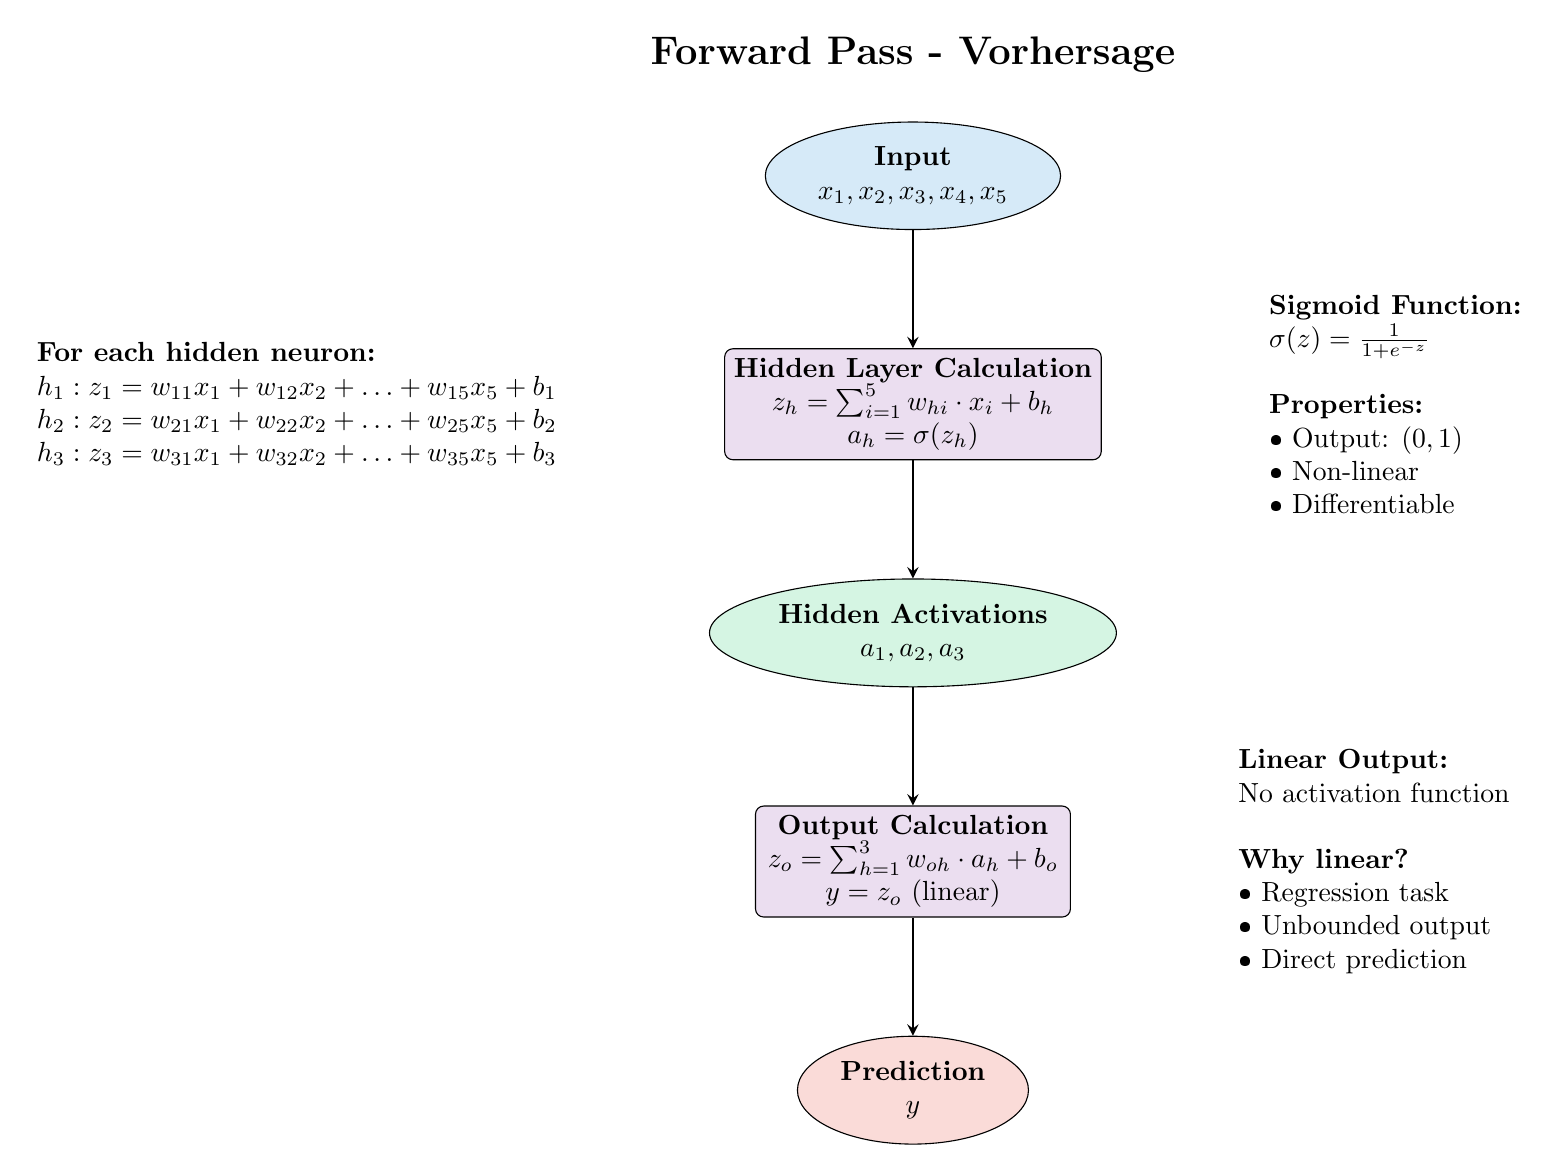
\begin{tikzpicture}[
    node distance=15mm,
    process/.style={rectangle, draw, rounded corners=3pt, minimum width=40mm, minimum height=8mm, align=center},
    data/.style={ellipse, draw, minimum width=25mm, minimum height=6mm, align=center},
    arrow/.style={->, >=stealth, thick}
]

% Forward Pass Flow
\node[data, fill=inputcolor!20] (input) {\textbf{Input}\\$x_1, x_2, x_3, x_4, x_5$};

\node[process, fill=calccolor!20, below=of input] (hidden_calc) {
    \textbf{Hidden Layer Calculation}\\
    $z_h = \sum_{i=1}^{5} w_{hi} \cdot x_i + b_h$\\
    $a_h = \sigma(z_h)$
};

\node[data, fill=hiddencolor!20, below=of hidden_calc] (hidden) {\textbf{Hidden Activations}\\$a_1, a_2, a_3$};

\node[process, fill=calccolor!20, below=of hidden] (output_calc) {
    \textbf{Output Calculation}\\
    $z_o = \sum_{h=1}^{3} w_{oh} \cdot a_h + b_o$\\
    $y = z_o$ (linear)
};

\node[data, fill=outputcolor!20, below=of output_calc] (output) {\textbf{Prediction}\\$y$};

% Arrows
\draw[arrow] (input) -- (hidden_calc);
\draw[arrow] (hidden_calc) -- (hidden);
\draw[arrow] (hidden) -- (output_calc);
\draw[arrow] (output_calc) -- (output);

% Side annotations
\node[right=20mm of hidden_calc, align=left] (sigmoid_note) {
    \textbf{Sigmoid Function:}\\
    $\sigma(z) = \frac{1}{1 + e^{-z}}$\\
    \\
    \textbf{Properties:}\\
    • Output: $(0, 1)$\\
    • Non-linear\\
    • Differentiable
};

\node[right=20mm of output_calc, align=left] (linear_note) {
    \textbf{Linear Output:}\\
    No activation function\\
    \\
    \textbf{Why linear?}\\
    • Regression task\\
    • Unbounded output\\
    • Direct prediction
};

% Mathematical details
\node[left=20mm of hidden_calc, align=left] (math_detail) {
    \textbf{For each hidden neuron:}\\
    $h_1: z_1 = w_{11}x_1 + w_{12}x_2 + \ldots + w_{15}x_5 + b_1$\\
    $h_2: z_2 = w_{21}x_1 + w_{22}x_2 + \ldots + w_{25}x_5 + b_2$\\
    $h_3: z_3 = w_{31}x_1 + w_{32}x_2 + \ldots + w_{35}x_5 + b_3$
};

% Title
\node[above=5mm of input, font=\Large\bfseries] {Forward Pass - Vorhersage};

\end{tikzpicture}
\end{document}
